\section{Conclusion and Future Works}
%Viscous is a bridge between \acrshort{mptcp} and \acrshort{quic}. It provides advantages from both the protocol i.e. it is multipath and provides better suitable for short-lived connections. It performs much better than \acrshort{mptcp} or \acrshort{tcp}. It also performs well enough for long-lived connections.
%
%\subsection{Future Works}
%Viscous is promising, but we need to do few improvement on it. It is required a better path scheduler. It is also needed to improve the congestion control algorithm. We need to implement the full mobility support.

The recent boost in the Internet traffic from various edge devices and IoT applications has resulted in poor network capacity utilization with the current TCP based transport protocols. In this study, we do a detailed analysis of the existing transport protocols, both theoretically and through thorough experiments, and observe that the existing transport protocols lack one or more of the three important features -- (a) mobility support, (b) capacity utilization for multi-homed devices, and (c) support of short lived real time flows over the network. Based on our analysis over the existing end-to-end transport protocols, we take an approach to develop a new application-transport wrapper or middleware, that can support the above three features. Although the task is challenging because of the dynamics of today's Internet traffic, we have developed the first baseline of a new protocol, called Viscous, which has a modular application programmability supports, and combines the bests from Google's QUIC and MPTCP protocols, as well as includes new features like decoupling of flow control and congestion control. We have designed and implemented the first version of Viscous for a Linux based platform, and thorough analysis of its performance results gives indication that the proposed protocol can significantly boost up the end-to-end transport performance, compared to standard TCP, MPTCP and QUIC. 

The next directions of this work are as follows. 
\begin{enumerate}
	\item [W1)] \textbf{Support of Application QoS}: The current design of Viscous use a naive channel and flow scheduling algorithms, those do not consider application QoS requirements. We plan to develop advanced channel and flow scheduling algorithms over Viscous, that can utilize environmental intelligence to support application QoS over the network. 
	\item [W2)] \textbf{Exploring Real Time Streaming over Viscous}: The current implementation of Viscous indicates that the worst case performance of Viscous is comparable with the standard TCP. Video streaming over the Internet is continuously gaining popularity, and the the streaming service providers use an adaptive streaming protocol over HTTP, that works on top of TCP. Our target is to explore the performance of real time multimedia streaming over Viscous, and then tune the protocols so that it can support QoS and quality of experience (QoE) for streaming over the Internet. 
	\item [W3)] \textbf{Large Scale Protocol Performance Testing} We plan to target for a large scale protocol performance testing for Viscous over open networking testbeds, such as the Geni testbed\footnote{\url{http://www.geni.net/} (last accessed: 24 April, 2017)}, that spans over the Internet. 
	\item [W4)] \textbf{Testbed Implementation for Viscous for IoT Communication} We have developed an IoT networking testbed using Raspberry Pi modules. We are now porting the Viscous implementation over the Raspberry Pi boards, and plan to go for a through testing under various network conditions. 
\end{enumerate} 

Fig.~\ref{fig:future} shows the projected milestones for the above works in the form of a Gnatt chart. Our target is to develop the next version of Viscous with the above features and test it over wide environments. 

\begin{figure}[!h]
	\centering
	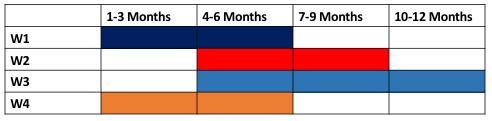
\includegraphics[width=0.6\linewidth]{img/future.png}
	\caption{Gnatt Chart for the Future Directions of the Work}
	\label{fig:future}
\end{figure}

\section*{Publications (Communicated)}

[1] Abhijit Mondal, Sourav Bhattacharjee, Sandip Chakraborty, ``Viscous: An End to End Protocol for Ubiquitous Communication over Internet of Everything", submitted to 42nd Annual IEEE Conference on Local Computer Networks (LCN 2017), Singapore, October 9-12, 2017